% =====================================================================
%  pop2vec / life-sequencing-dutch  --  Codebase & Pipeline Report
%  Compile with:  pdflatex pipeline_report.tex   (run twice for refs)
% =====================================================================
\documentclass[11pt,a4paper]{article}

\usepackage[margin=2.4cm]{geometry}
\usepackage[T1]{fontenc}
\usepackage[utf8]{inputenc}
\usepackage{lmodern}
\usepackage{amsmath,amssymb}
\usepackage{booktabs}
\usepackage{array}
\usepackage{enumitem}
\usepackage{xcolor}
\usepackage{tikz}
\usetikzlibrary{arrows.meta,positioning,fit,calc,shapes.geometric,backgrounds,matrix}
\usepackage[colorlinks=true,linkcolor=blue!60!black,urlcolor=blue!60!black]{hyperref}
\usepackage{graphicx}
\usepackage{caption}
\captionsetup{font=small,labelfont=bf}

% ---------- colors ----------
\definecolor{cData}{RGB}{221,235,247}   % light blue  (data)
\definecolor{cProc}{RGB}{226,239,218}   % light green (scripts/processes)
\definecolor{cModel}{RGB}{252,228,214}  % light orange (model blocks)
\definecolor{cHead}{RGB}{237,226,246}   % light purple (heads / decoders)
\definecolor{cLoss}{RGB}{255,242,204}   % light yellow (losses / outputs)
\definecolor{cGrey}{RGB}{237,237,237}

% ---------- tikz styles ----------
\tikzset{
  data/.style={draw=blue!50!black, fill=cData, rounded corners=2pt,
               minimum height=8mm, align=center, font=\small},
  proc/.style={draw=green!40!black, fill=cProc, rounded corners=2pt,
               minimum height=8mm, align=center, font=\small},
  model/.style={draw=orange!60!black, fill=cModel, rounded corners=2pt,
               minimum height=8mm, align=center, font=\small},
  head/.style={draw=violet!60!black, fill=cHead, rounded corners=2pt,
               minimum height=8mm, align=center, font=\small},
  loss/.style={draw=yellow!40!black, fill=cLoss, rounded corners=2pt,
               minimum height=8mm, align=center, font=\small},
  tok/.style={draw=black!60, fill=cGrey, minimum width=13mm, minimum height=6.5mm,
              align=center, font=\scriptsize, inner sep=1pt},
  tokm/.style={tok, fill=red!20},
  toks/.style={tok, fill=blue!15},
  arr/.style={-{Stealth[length=2.4mm]}, thick},
  lbl/.style={font=\scriptsize\itshape, text=black!70},
}

\newcommand{\file}[1]{\texttt{\small #1}}
\newcommand{\code}[1]{\texttt{\small #1}}

\title{\textbf{Life Sequences as Language:\\
A Complete Guide to the \code{pop2vec} LLM Pipeline}\\[2mm]
\large BERT-style (MLM) and GPT-style (AR) transformers over Dutch registry life-event data}
\author{Documentation generated from the codebase\\
\small repository: \code{life-sequencing-dutch}, module: \code{pop2vec/llm}}
\date{\today}

\begin{document}
\maketitle

\begin{abstract}
\noindent
This report explains, end to end, how the \code{pop2vec} codebase turns Dutch
administrative registry data into \emph{life sequences}, pretrains a transformer
on them (extending \emph{life2vec}, arXiv:2306.03009), and produces downstream
predictions in two ways: (1) \textbf{static} --- freeze the pretrained encoder,
export one embedding per person, and train a small MLP on those embeddings; and
(2) \textbf{finetuned} --- attach a task head to the pretrained encoder and train
the whole network per task. The same encoder supports two pretraining objectives
selected by the \code{training\_task} hyperparameter: \code{mlm} (BERT-style
masked language modelling, the default) and \code{ar\_lm} (GPT-style
autoregressive next-token prediction with causal attention). Every section
includes diagrams in the spirit of the BERT and ``Attention is All You Need''
papers, and maps each concept to the exact file and function that implements it.
\end{abstract}

\tableofcontents
\clearpage

% =====================================================================
\section{The Big Picture}
% =====================================================================

The core idea inherited from life2vec: \textbf{treat a person's life as a
document}. Every life event (a job change, a move, a hospital visit, a marriage)
becomes a \emph{sentence}; every attribute of the event becomes a \emph{token}
(e.g.\ \code{income\_percentile\_87}). A transformer is pretrained on millions of
such documents, exactly like BERT/GPT on text, and the learned representations
are then used to predict life outcomes.

\begin{figure}[h!]
\centering
\resizebox{0.98\textwidth}{!}{%
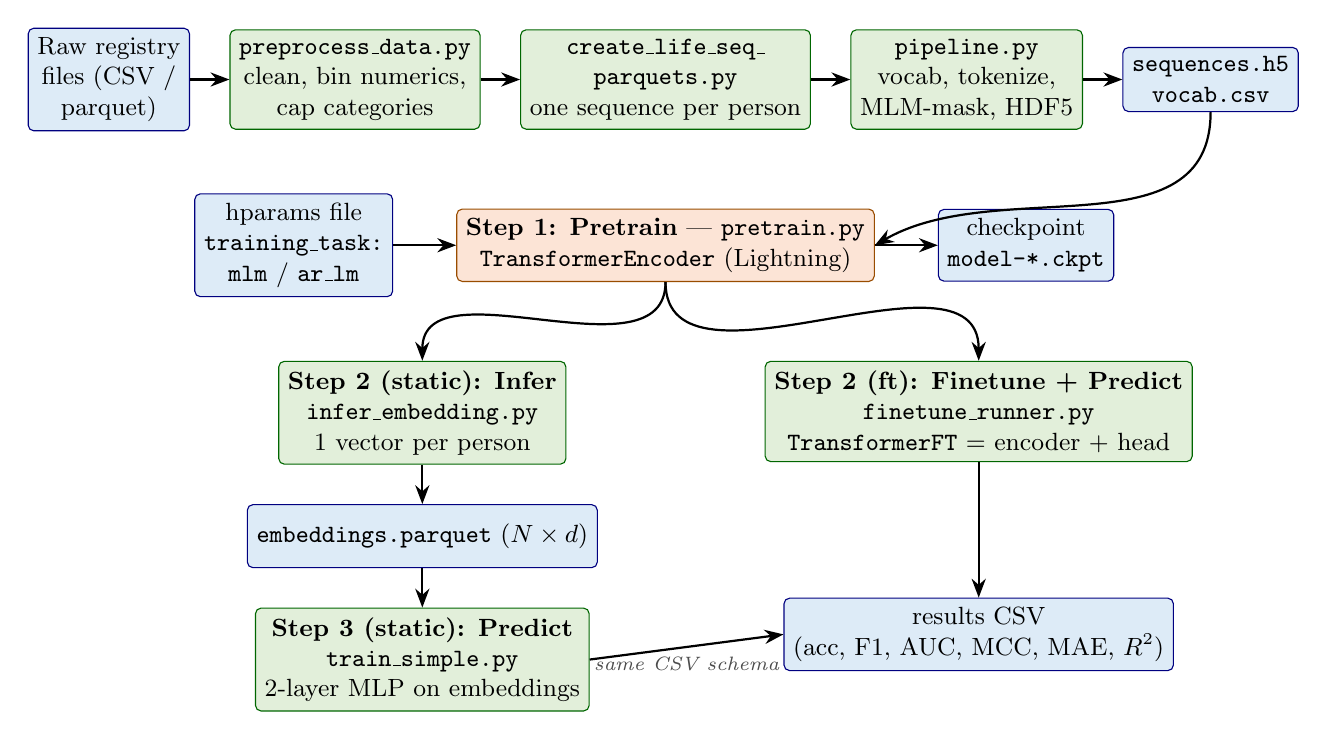
\begin{tikzpicture}[node distance=6mm and 5mm]
  % --- stage 1: data prep (top row)
  \node[data]  (raw)   {Raw registry\\ files (CSV /\\ parquet)};
  \node[proc,  right=of raw] (prep)  {\file{preprocess\_data.py}\\ clean, bin numerics,\\ cap categories};
  \node[proc,  right=of prep] (seq)  {\file{create\_life\_seq\_}\\\file{parquets.py}\\ one sequence per person};
  \node[proc,  right=of seq] (pipe)  {\file{pipeline.py}\\ vocab, tokenize,\\ MLM-mask, HDF5};
  \node[data,  right=of pipe] (h5)   {\code{sequences.h5}\\ \code{vocab.csv}};

  % --- stage 2: pretraining (middle row)
  \node[model, below=10mm of seq] (pretrain) {\textbf{Step 1: Pretrain} --- \file{pretrain.py}\\ \code{TransformerEncoder} (Lightning)};
  \node[data, left=8mm of pretrain]  (hp)  {hparams file\\ \code{training\_task:}\\ \code{mlm} / \code{ar\_lm}};
  \node[data, right=8mm of pretrain] (ckpt) {checkpoint\\ \code{model-*.ckpt}};

  % --- stage 3a: static (bottom left)
  \node[proc, below left=10mm and -14mm of pretrain] (infer) {\textbf{Step 2 (static): Infer}\\ \file{infer\_embedding.py}\\ 1 vector per person};
  \node[data, below=5mm of infer] (emb) {\code{embeddings.parquet} ($N \times d$)};
  \node[proc, below=5mm of emb] (mlp) {\textbf{Step 3 (static): Predict}\\ \file{train\_simple.py}\\ 2-layer MLP on embeddings};

  % --- stage 3b: finetune (bottom right)
  \node[proc, below right=10mm and -14mm of pretrain] (ft) {\textbf{Step 2 (ft): Finetune + Predict}\\ \file{finetune\_runner.py}\\ \code{TransformerFT} = encoder + head};
  \node[data, below=17.2mm of ft] (res) {results CSV\\ (acc, F1, AUC, MCC, MAE, $R^2$)};

  % arrows
  \draw[arr] (raw) -- (prep);
  \draw[arr] (prep) -- (seq);
  \draw[arr] (seq) -- (pipe);
  \draw[arr] (pipe) -- (h5);
  \draw[arr] (h5.south) to[out=-90,in=30] (pretrain.east);
  \draw[arr] (hp) -- (pretrain);
  \draw[arr] (pretrain) -- (ckpt);
  \draw[arr] (pretrain.south) to[out=-90,in=90] (infer.north);
  \draw[arr] (pretrain.south) to[out=-90,in=90] (ft.north);
  \draw[arr] (infer) -- (emb);
  \draw[arr] (emb) -- (mlp);
  \draw[arr] (ft) -- (res);
  \draw[arr] (mlp.east) -- node[lbl,below]{same CSV schema} (res.west);
\end{tikzpicture}}
\caption{The full pipeline. The two downstream routes (\emph{static} left,
\emph{finetuned} right) both start from the same pretrained checkpoint and
report results in an identical CSV schema, so numbers are directly comparable.}
\label{fig:pipeline}
\end{figure}

\paragraph{Your workflow, confirmed.} The four entry points you listed are
exactly right:
\begin{enumerate}[nosep]
  \item \textbf{Pretrain}: \file{pop2vec/llm/src/new\_code/pretrain.py}
  \item[2a.] \textbf{Static, infer}: \file{pop2vec/llm/src/new\_code/infer\_embedding.py}
  \item[2b.] \textbf{Finetune + predict}: \file{pop2vec/llm/src/new\_code/finetune\_runner.py}
  \item[3a.] \textbf{Static, predict}: \file{pop2vec/llm/src/new\_code/train\_simple.py}
\end{enumerate}
The only step upstream of these is data preparation (Section~\ref{sec:data}),
which produces the tokenized HDF5 file and the vocabulary CSV that
\file{pretrain.py} consumes.

% =====================================================================
\section{Data: From Registry Tables to Token Sequences}\label{sec:data}
% =====================================================================

\subsection{Attribute preprocessing (\file{preprocess\_data.py})}
Each raw table (CSV or parquet, one row per event per person, keyed by
\code{RINPERSOON}) is normalized so that every column becomes a small
categorical alphabet:
\begin{itemize}[nosep]
  \item \textbf{Numeric columns} are converted to \textbf{percentiles}
        (\code{transform\_to\_percentiles}), so ``income = 43{,}210~EUR'' becomes
        ``income is in percentile bucket 87''. This is what makes a continuous
        value usable as a token.
  \item \textbf{Categorical columns} keep only the \textbf{top 100} most frequent
        values; the rest are renamed \code{Others}
        (\code{replace\_less\_frequent}).
  \item Missing values become the literal token \code{MISSING}; rows without the
        two time columns (\code{age}, \code{days\_since\_first}) are dropped;
        columns matching restricted substrings are removed.
\end{itemize}
The result: every event attribute has at most $\sim$100 distinct values, keeping
the final vocabulary compact.

\subsection{Sequence construction and tokenization (\file{pipeline.py} + \file{tasks/mlm.py})}
For each person, events are ordered in time and encoded by
\code{MLM.encode\_document()}:
\begin{enumerate}[nosep]
  \item A \textbf{prefix sentence} is built:
        \code{[CLS]} $+$ background tokens (fixed characteristics such as gender,
        birth year, origin) $+$ \code{[SEP]}.
  \item Every \textbf{event} becomes a sentence of tokens (one token per
        attribute, spelled \code{attribute\_value}) terminated by \code{[SEP]}.
  \item If the whole document exceeds \code{max\_length} (512 in the standard
        config), the \emph{oldest} events are dropped --- the code keeps the most
        \emph{recent} events that fit (suffix truncation).
  \item People with fewer than 5 events (\code{MIN\_EVENT\_THRESHOLD}) are
        skipped.
\end{enumerate}

Each sequence is stored as a $4 \times L_{\max}$ integer matrix
(\code{input\_ids}), i.e.\ \textbf{four parallel streams} per token position:

\begin{figure}[h!]
\centering
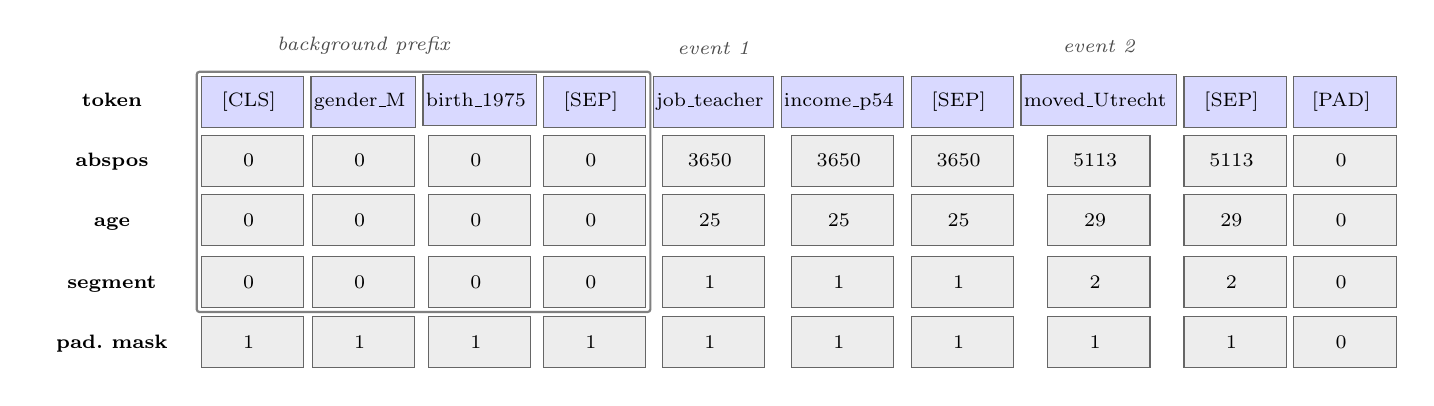
\begin{tikzpicture}[node distance=0mm]
  \matrix (m) [matrix of nodes, nodes={tok}, column sep=0.8mm, row sep=0.8mm,
               row 1/.style={nodes={toks}},
               ampersand replacement=\&] {
    |[fill=white,draw=none,minimum width=20mm,align=right]| \textbf{token} \&
      {[CLS]} \& gender\_M \& birth\_1975 \& {[SEP]} \& job\_teacher \& income\_p54 \& {[SEP]} \& moved\_Utrecht \& {[SEP]} \& {[PAD]} \\
    |[fill=white,draw=none,align=right]| \textbf{abspos} \&
      0 \& 0 \& 0 \& 0 \& 3650 \& 3650 \& 3650 \& 5113 \& 5113 \& 0 \\
    |[fill=white,draw=none,align=right]| \textbf{age} \&
      0 \& 0 \& 0 \& 0 \& 25 \& 25 \& 25 \& 29 \& 29 \& 0 \\
    |[fill=white,draw=none,align=right]| \textbf{segment} \&
      0 \& 0 \& 0 \& 0 \& 1 \& 1 \& 1 \& 2 \& 2 \& 0 \\
    |[fill=white,draw=none,align=right]| \textbf{pad.\ mask} \&
      1 \& 1 \& 1 \& 1 \& 1 \& 1 \& 1 \& 1 \& 1 \& 0 \\
  };
  \node[lbl, above=1.5mm of m-1-3] {background prefix};
  \node[lbl, above=1.5mm of m-1-6] {event 1};
  \node[lbl, above=1.5mm of m-1-9] {event 2};
  \draw[black!50, thick, rounded corners=1pt] ($(m-1-2.north west)+(-0.5mm,0.5mm)$) rectangle ($(m-4-5.south east)+(0.5mm,-0.5mm)$);
\end{tikzpicture}
\caption{One person's encoded life sequence (toy example). \code{input\_ids} has
shape $(4, L_{\max})$: token ids, absolute position in days
(\code{abspos}), age at the event, and segment id. All tokens of the same event
share the same abspos/age/segment. The prefix carries zeros for all three time
streams. \code{padding\_mask} marks real tokens.}
\label{fig:input}
\end{figure}

\noindent The encoded corpus is written to HDF5 with these datasets:
\begin{center}\small
\begin{tabular}{@{}llp{8.2cm}@{}}
\toprule
\textbf{dataset} & \textbf{shape} & \textbf{meaning} \\
\midrule
\code{input\_ids}         & $(N,4,L_{\max})$ & the 4-stream input above (token stream masked if MLM-encoded) \\
\code{padding\_mask}      & $(N,L_{\max})$   & 1 = real token, 0 = padding \\
\code{original\_sequence} & $(N,L_{\max})$   & unmasked token ids (MLM files only) \\
\code{target\_tokens}     & $(N,T)$          & true ids of masked positions, $-1$-padded (MLM only) \\
\code{target\_pos}        & $(N,T)$          & positions that were masked (MLM only) \\
\code{target\_cls}        & $(N,)$           & sequence-order label 0/1/2 (MLM only, Sec.~\ref{sec:mlm}) \\
\code{sequence\_id}       & $(N,)$           & \code{RINPERSOON} of the person \\
\bottomrule
\end{tabular}
\end{center}

\paragraph{Vocabulary.} \code{CustomVocabulary} scans all data files and writes
\code{vocab.csv} with columns \code{TOKEN, CATEGORY, ID}. IDs $0$--$8$ are
reserved general tokens; the important ones are \code{[PAD]}$=0$, plus
\code{[CLS]}, \code{[SEP]}, \code{[UNK]}, \code{[MASK]}, and (in real data) a
death token \code{[death]\_[death]}. \file{pretrain.py} reads
\code{vocab\_size} as simply the number of rows of this CSV and looks up the
special ids with \code{load\_special\_ids()} (\file{utils.py}).

\paragraph{Data loading.} \file{load\_data.py} provides several dataset classes;
the one used by pretraining and inference is \code{CustomLazyHDF5Dataset}: it
opens the HDF5 lazily (one handle per worker), and splits
\textbf{validation = first \code{num\_val\_items} rows}, training = the rest
(inference mode returns all rows). Finetuning uses \code{FineTuneLazyDataset},
which additionally joins the HDF5 rows with a label file (CSV/parquet keyed by
\code{RINPERSOON}) and keeps only the intersection.

% =====================================================================
\section{Model Architecture}\label{sec:model}
% =====================================================================

The encoder (class \code{Transformer} in \file{transformer/transformer.py}) is a
standard pre-norm/ReZero transformer stack, with two life2vec-specific twists:
\textbf{Time2Vec temporal embeddings} and \textbf{Performer (FAVOR+) attention}
with local attention heads.

\begin{figure}[h!]
\centering
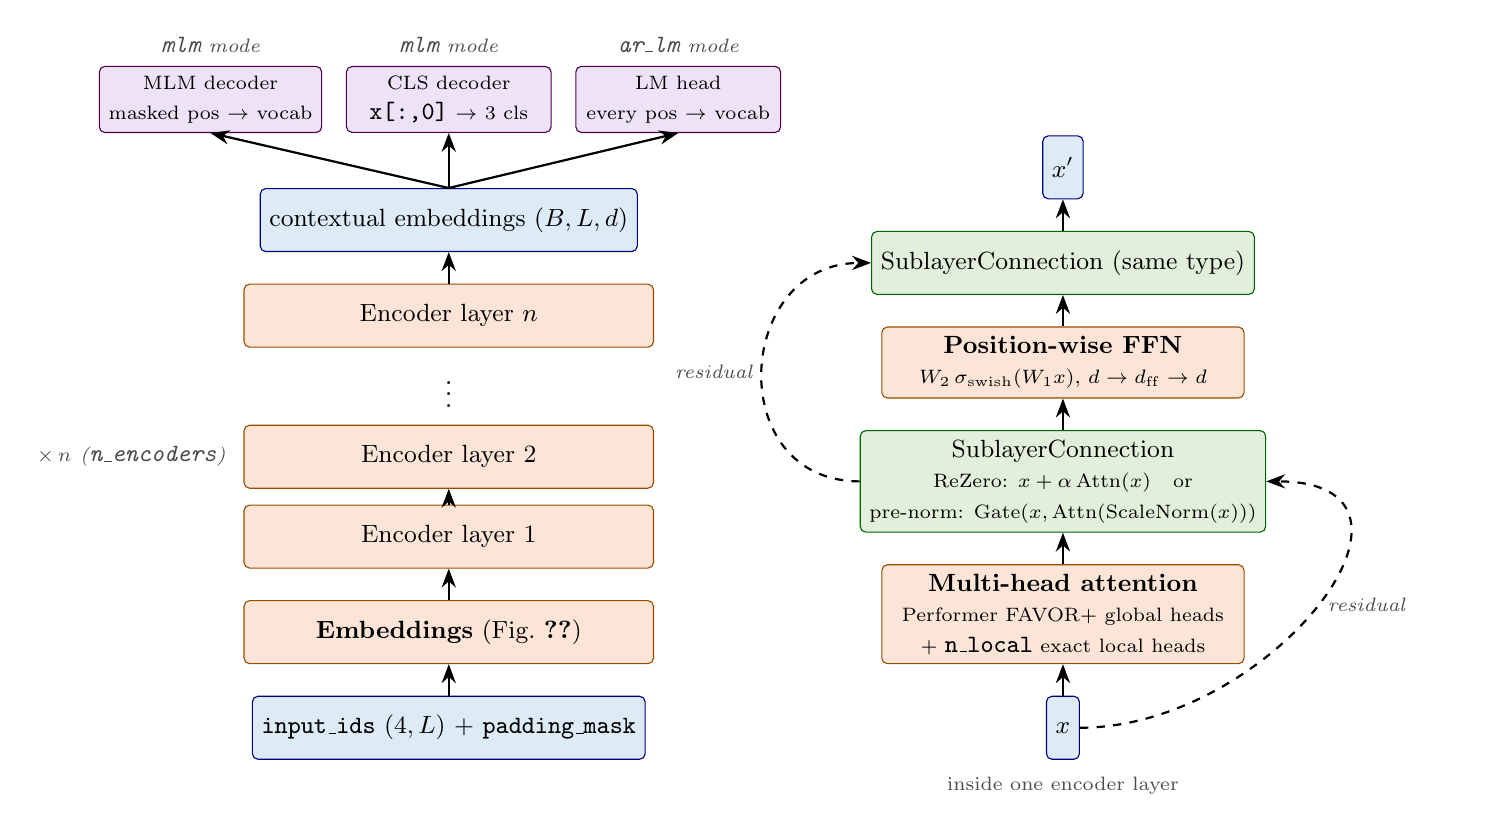
\begin{tikzpicture}[node distance=4mm and 12mm]
  % ---- left: whole stack ----
  \node[data] (inp) {\code{input\_ids} $(4,L)$ + \code{padding\_mask}};
  \node[model, above=of inp, minimum width=52mm] (emb) {\textbf{Embeddings} (Fig.~\ref{fig:emb})};
  \node[model, above=of emb, minimum width=52mm] (enc1) {Encoder layer 1};
  \node[model, above=2mm of enc1, minimum width=52mm] (enc2) {Encoder layer 2};
  \node[draw=none, above=1mm of enc2] (dots) {$\vdots$};
  \node[model, above=1mm of dots, minimum width=52mm] (encN) {Encoder layer $n$};
  \node[data, above=of encN] (out) {contextual embeddings $(B,L,d)$};
  \draw[arr] (inp) -- (emb);
  \draw[arr] (emb) -- (enc1);
  \draw[arr] (enc1) -- (enc2);
  \draw[arr] (encN) -- (out);
  \node[lbl, left=1mm of enc2] {$\times\, n$ (\code{n\_encoders})};

  % heads
  \node[head, above=7mm of out, minimum width=26mm] (clsh) {\scriptsize CLS decoder\\ \scriptsize \code{x[:,0]} $\to$ 3 cls};
  \node[head, left=3mm of clsh, minimum width=26mm] (mlmh) {\scriptsize MLM decoder\\ \scriptsize masked pos $\to$ vocab};
  \node[head, right=3mm of clsh, minimum width=26mm] (lmh) {\scriptsize LM head\\ \scriptsize every pos $\to$ vocab};
  \draw[arr] (out.north) -- (mlmh.south);
  \draw[arr] (out.north) -- (clsh.south);
  \draw[arr] (out.north) -- (lmh.south);
  \node[lbl, above=0.5mm of mlmh] {\code{mlm} mode};
  \node[lbl, above=0.5mm of clsh] {\code{mlm} mode};
  \node[lbl, above=0.5mm of lmh] {\code{ar\_lm} mode};

  % ---- right: inside one encoder layer ----
  \begin{scope}[xshift=78mm]
    \node[data] (x0) {$x$};
    \node[model, above=of x0, minimum width=46mm] (att) {\textbf{Multi-head attention}\\
      \scriptsize Performer FAVOR+ global heads\\ \scriptsize $+$ \code{n\_local} exact local heads};
    \node[proc, above=of att, minimum width=46mm] (sub1) {SublayerConnection\\ \scriptsize ReZero: $x + \alpha\,\mathrm{Attn}(x)$\quad or\\ \scriptsize pre-norm: $\mathrm{Gate}(x, \mathrm{Attn}(\mathrm{ScaleNorm}(x)))$};
    \node[model, above=of sub1, minimum width=46mm] (ffn) {\textbf{Position-wise FFN}\\ \scriptsize $W_2\,\sigma_{\text{swish}}(W_1 x)$, $d \to d_{\mathrm{ff}} \to d$};
    \node[proc, above=of ffn, minimum width=46mm] (sub2) {SublayerConnection (same type)};
    \node[data, above=of sub2] (x1) {$x'$};
    \draw[arr] (x0) -- (att);
    \draw[arr] (att) -- (sub1);
    \draw[arr] (sub1) -- (ffn);
    \draw[arr] (ffn) -- (sub2);
    \draw[arr] (sub2) -- (x1);
    \draw[arr, dashed] (x0.east) to[out=0,in=0, looseness=1.6] node[lbl,right]{residual} (sub1.east);
    \draw[arr, dashed] (sub1.west) to[out=180,in=180, looseness=1.6] node[lbl,left]{residual} (sub2.west);
    \node[lbl, below=1mm of x0] {\emph{inside one encoder layer}};
  \end{scope}
\end{tikzpicture}
\caption{Left: the full model (\code{TransformerEncoder} in
\file{transformer/models.py}). One shared encoder; the heads differ by
pretraining mode. Right: one \code{EncoderLayer}
(\file{transformer/transformer\_utils.py}). Between layers, padded positions are
re-zeroed via \code{einsum("bsh,bs->bsh", x, padding\_mask)}.}
\label{fig:arch}
\end{figure}

\subsection{Embedding block: how a token meets its time}
Instead of BERT's learned position embeddings, each token embedding is combined
with \textbf{Time2Vec} encodings of \emph{age} and \emph{calendar time}
(\code{abspos}), and a small \emph{segment} embedding. Time2Vec, implemented
in \file{transformer/embeddings.py}, maps a scalar $\tau$ to a $d$-dimensional
vector
\[
\mathrm{t2v}(\tau) \;=\; \big[\, f(\tau w + b) \,\|\, \tau w_0 + b_0 \,\big],
\qquad f = \cos \text{ (age)}, \; f = \sin \text{ (abspos)},
\]
i.e.\ $d-1$ periodic features plus one linear feature, with learned frequencies.
Each additive term enters through its own \textbf{ReZero residual}
$x \mapsto x + \alpha \cdot \mathrm{t2v}$ with a learned scalar $\alpha$
initialized at $0$ --- so the model \emph{starts as a pure bag-of-tokens} and
learns how much time information to inject.

\begin{figure}[h!]
\centering
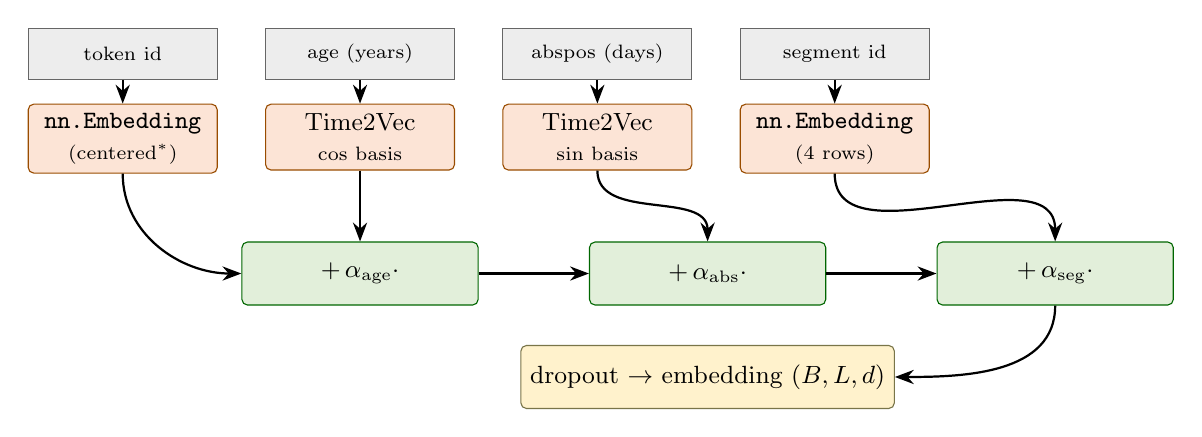
\begin{tikzpicture}[node distance=3mm and 6mm]
  \node[tok, minimum width=24mm] (t) {token id};
  \node[tok, minimum width=24mm, right=of t] (a) {age (years)};
  \node[tok, minimum width=24mm, right=of a] (p) {abspos (days)};
  \node[tok, minimum width=24mm, right=of p] (s) {segment id};

  \node[model, below=of t, minimum width=24mm]  (te) {\code{nn.Embedding}\\ \scriptsize (centered$^{*}$)};
  \node[model, below=of a, minimum width=24mm]  (ae) {Time2Vec\\ \scriptsize $\cos$ basis};
  \node[model, below=of p, minimum width=24mm]  (pe) {Time2Vec\\ \scriptsize $\sin$ basis};
  \node[model, below=of s, minimum width=24mm]  (se) {\code{nn.Embedding}\\ \scriptsize (4 rows)};

  \node[proc, below=9mm of ae, minimum width=30mm] (r1) {$+\,\alpha_{\mathrm{age}}\cdot$};
  \node[proc, right=14mm of r1, minimum width=30mm] (r2) {$+\,\alpha_{\mathrm{abs}}\cdot$};
  \node[proc, right=14mm of r2, minimum width=30mm] (r3) {$+\,\alpha_{\mathrm{seg}}\cdot$};
  \node[loss, below=5mm of r2, minimum width=40mm] (drop) {dropout $\to$ embedding $(B,L,d)$};

  \draw[arr] (t) -- (te); \draw[arr] (a) -- (ae); \draw[arr] (p) -- (pe); \draw[arr] (s) -- (se);
  \draw[arr] (te.south) to[out=-90,in=180] (r1.west);
  \draw[arr] (ae) -- (r1);
  \draw[arr] (r1) -- (r2);
  \draw[arr] (pe.south) to[out=-90,in=90] (r2.north);
  \draw[arr] (r2) -- (r3);
  \draw[arr] (se.south) to[out=-90,in=90] (r3.north);
  \draw[arr] (r3.south) to[out=-90,in=0] (drop.east);
\end{tikzpicture}
\caption{The embedding block (\code{Embeddings.forward}). ReZero scalars
$\alpha$ start at 0. $^{*}$If \code{parametrize\_emb} is true, the token
embedding matrix is mean-centered on every forward pass (ignoring PAD and
placeholder ids), optionally $\ell_2$-normalized. The first 5 positions of each
Time2Vec output are zeroed (\code{pos[:, :5] *= 0}) so the background prefix
stays time-free.}
\label{fig:emb}
\end{figure}

\subsection{Attention: Performer with local heads}
Full $O(L^2)$ softmax attention is \emph{deprecated} in this codebase
(\file{transformer/attention.py} raises if you ask for it). Instead,
\code{attention\_type: performer} uses the FAVOR+ approximation, implemented
in \file{transformer/performer.py} as a wrapper around the
\code{performer\_pytorch} package:
\[
\mathrm{Attn}(Q,K,V) \approx \hat{D}^{-1}\big(\phi(Q)\,(\phi(K)^\top V)\big),
\qquad \phi = \text{positive random features (\code{num\_random\_features})},
\]
which is linear in sequence length. Of the \code{n\_heads} heads,
\code{n\_local} are \textbf{exact sliding-window heads} (window
\code{local\_window\_size}) that capture short-range structure (within-event and
neighbouring-event patterns), and the remaining global heads use FAVOR+ for
long-range structure. For the GPT mode, the same module runs with
\code{causal\_attn: true} so each position can only attend to its past.
Projection matrices are periodically redrawn during training
(\code{redraw\_projection\_matrix}, called at each epoch end).

\subsection{Heads}
\begin{description}[nosep]
  \item[MLM decoder (\code{MaskedLanguageModel}).] Gathers the hidden vectors at
    the masked positions (\code{target\_pos}), applies
    $\mathrm{dropout} \to \tanh(Vx) \to \ell_2\text{-norm} \to g \cdot W_{\text{out}}$,
    where $W_{\text{out}}$ is \textbf{weight-tied} to the token embedding matrix
    (\code{weight\_tying: wt}) and $g$ is a learned temperature initialized to
    $\sqrt{d}$. Output: logits over the vocabulary for each masked slot.
  \item[CLS decoder (\code{CLS\_DecoderS}).] Takes the hidden state of position
    0 (the \code{[CLS]} token), applies
    $\mathrm{Linear}\to\mathrm{swish}\to\mathrm{ScaleNorm}\to\mathrm{dropout}\to\mathrm{Linear}$
    to 3 classes (Sec.~\ref{sec:mlm} explains the 3 classes).
  \item[AR LM head (\code{lm\_head}).] A single bias-free linear layer
    $d \to |V|$, weight-tied to the token embedding, applied to \emph{every}
    position.
\end{description}

\subsection{Reference hyperparameters}
From \file{new\_code/regular\_hparams.txt}, the ``small/base'' config; the
\code{medium}, \code{medium2x} and \code{large} files in the same folder scale
these up:
\begin{center}\small
\begin{tabular}{@{}llll@{}}
\toprule
\code{hidden\_size} $d$ & 280 & \code{n\_encoders} & 5 \\
\code{hidden\_ff} $d_{\mathrm{ff}}$ & 2210 & \code{n\_heads} & 10 \\
\code{n\_local} (exact heads) & 7 & \code{local\_window\_size} & 38 \\
\code{num\_random\_features} & 436 & \code{max\_length} & 512 \\
\code{norm\_type} & rezero & \code{hidden\_act} & swish \\
dropouts (att/ff/dec/emb) & 0.1 & \code{weight\_tying} & wt \\
\code{learning\_rate} & 5e-3 (OneCycle) & \code{weight\_decay} & 0.01 \\
\bottomrule
\end{tabular}
\end{center}

% =====================================================================
\section{Step 1 --- Pretraining (\file{pretrain.py})}\label{sec:pretrain}
% =====================================================================

\code{pretrain.py} is a thin PyTorch-Lightning launcher: it reads the hparams
file, builds train/val dataloaders over the HDF5, instantiates
\code{TransformerEncoder}, and calls \code{Trainer.fit}. The one switch that
changes everything is
\begin{center}
\code{training\_task: mlm} \quad (default, BERT-style) \qquad vs. \qquad
\code{training\_task: ar\_lm} \quad (GPT-style).
\end{center}

\subsection{BERT mode: masked LM + sequence-order CLS task}\label{sec:mlm}
Masking is done \textbf{once, offline}, by \file{pipeline.py} when the HDF5 is
created (not on the fly): \code{mlm\_mask()} in \file{tasks/mlm.py} selects
\code{mask\_ratio}$\,=30\%$ of the real tokens (never \code{[SEP]}/\code{[UNK]},
never position 0) and, of those selected:
$\sim$80\% are replaced by \code{[MASK]}, $\sim$10\% are replaced by a random
non-special token, and $\sim$10\% are left unchanged --- BERT's classic 80/10/10,
with an optional ``smart masking'' variant that samples the random replacement
from the \emph{same attribute category}. An alternative \code{masking: event}
mode masks whole events (sentences) instead of individual tokens.

In addition to MLM, life2vec's auxiliary \textbf{sequence-order task} is kept:
with probability 0.05 the event order of the document is \emph{reversed}
(label 1), with probability 0.05 it is \emph{shuffled} (label 2), otherwise it
is intact (label 0); the label is stored as \code{target\_cls} and predicted
from the \code{[CLS]} position. This forces the \code{[CLS]} summary to be
sensitive to temporal coherence. Because the classes are imbalanced
(90/5/5), the CLS loss uses inverse-frequency class weights
(\code{cls\_a} $=[1/0.9,\,1/0.1,\,1/0.1]$) and label smoothing 0.1.

\begin{figure}[h!]
\centering
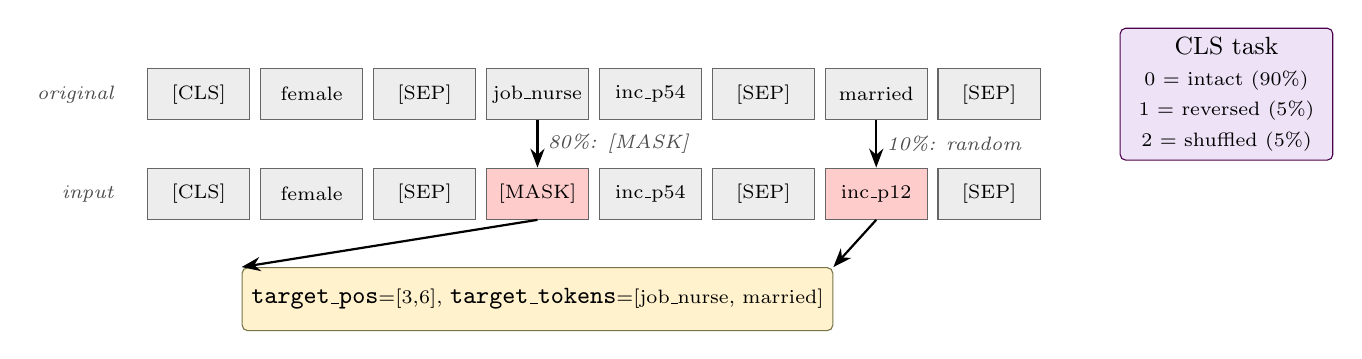
\begin{tikzpicture}[node distance=1.2mm and 1.2mm]
  % original
  \node[tok] (o1) {[CLS]};
  \node[tok, right=of o1] (o2) {female};
  \node[tok, right=of o2] (o3) {[SEP]};
  \node[tok, right=of o3] (o4) {job\_nurse};
  \node[tok, right=of o4] (o5) {inc\_p54};
  \node[tok, right=of o5] (o6) {[SEP]};
  \node[tok, right=of o6] (o7) {married};
  \node[tok, right=of o7] (o8) {[SEP]};
  \node[lbl, left=3mm of o1] {original};

  % masked
  \node[tok, below=6mm of o1] (m1) {[CLS]};
  \node[tok,  right=of m1] (m2) {female};
  \node[tok,  right=of m2] (m3) {[SEP]};
  \node[tokm, right=of m3] (m4) {[MASK]};
  \node[tok,  right=of m4] (m5) {inc\_p54};
  \node[tok,  right=of m5] (m6) {[SEP]};
  \node[tokm, right=of m6] (m7) {inc\_p12};
  \node[tok,  right=of m7] (m8) {[SEP]};
  \node[lbl, left=3mm of m1] {input};

  \draw[arr] (o4) -- node[lbl,right]{80\%: [MASK]} (m4);
  \draw[arr] (o7) -- node[lbl,right]{10\%: random} (m7);

  % targets
  \node[loss, below=6mm of m4, minimum width=34mm] (t1) {\scriptsize \code{target\_pos}=[3,6], \code{target\_tokens}=[job\_nurse, married]};
  \draw[arr] (m4.south) -- (t1.north west);
  \draw[arr] (m7.south) -- (t1.north east);

  % cls side
  \node[head, right=10mm of o8, minimum width=27mm] (cls) {CLS task\\ \scriptsize 0 = intact (90\%)\\ \scriptsize 1 = reversed (5\%)\\ \scriptsize 2 = shuffled (5\%)};
\end{tikzpicture}
\caption{MLM encoding, done offline in \file{pipeline.py}. The model must
recover the true tokens at \code{target\_pos}; simultaneously the \code{[CLS]}
head must detect whether the event order was tampered with.}
\label{fig:mlm}
\end{figure}

\noindent The training loss (\code{TransformerEncoder.training\_step}) is the
life2vec weighted sum:
\[
\mathcal{L} \;=\; 0.8\,\underbrace{\mathrm{CE}\big(\text{MLM logits},\,
\text{target\_tokens}\big)}_{\text{ignore\_index}=0}
\;+\; 0.2\,\underbrace{\mathrm{CE}_{w}\big(\text{CLS logits},\,
\text{target\_cls}\big)}_{\text{class-weighted, smoothed}}.
\]
Logged metrics include top-5 macro accuracy/precision/recall/F1 over the
vocabulary, CLS accuracy/F1, and perplexity $e^{\mathcal{L}_{\mathrm{MLM}}}$.

\subsection{GPT mode: autoregressive next-token prediction}
For \code{training\_task: ar\_lm}, three things change:
\begin{enumerate}[nosep]
  \item \textbf{Data}: the HDF5 is read with \code{mlm\_encoded=False} (the raw,
        unmasked token stream), and the collate function
        \code{collate\_autoreg()} (\file{load\_data.py}) builds the shifted
        (input, target) pairs on the fly.
  \item \textbf{Attention}: \code{causal\_attn: true} makes every head (FAVOR+
        and local) causal.
  \item \textbf{Head/loss}: the tied \code{lm\_head} predicts the next token at
        every position; loss is cross-entropy with \code{ignore\_index=0}
        (PAD), and perplexity is logged (clamped at $e^{20}$ for safety).
\end{enumerate}
\code{collate\_autoreg} also implements a life-specific rule: each sequence is
\textbf{truncated at the first death token} (inclusive) --- there is nothing to
predict after death.

\begin{figure}[h!]
\centering
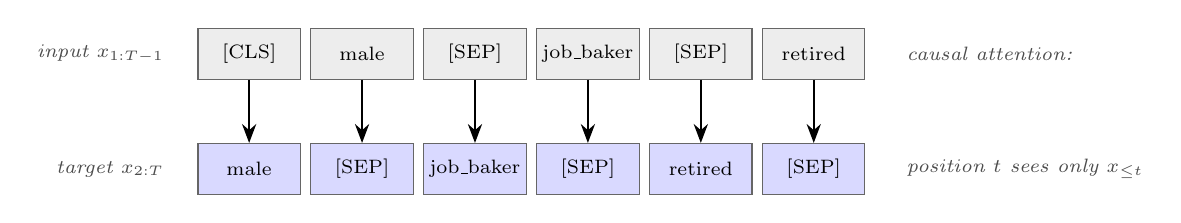
\begin{tikzpicture}[node distance=1.2mm and 1.2mm]
  \node[tok] (i1) {[CLS]};
  \node[tok, right=of i1] (i2) {male};
  \node[tok, right=of i2] (i3) {[SEP]};
  \node[tok, right=of i3] (i4) {job\_baker};
  \node[tok, right=of i4] (i5) {[SEP]};
  \node[tok, right=of i5] (i6) {retired};
  \node[lbl, left=3mm of i1] {input $x_{1:T-1}$};

  \node[toks, below=8mm of i1] (t1) {male};
  \node[toks, right=of t1] (t2) {[SEP]};
  \node[toks, right=of t2] (t3) {job\_baker};
  \node[toks, right=of t3] (t4) {[SEP]};
  \node[toks, right=of t4] (t5) {retired};
  \node[toks, right=of t5] (t6) {[SEP]};
  \node[lbl, left=3mm of t1] {target $x_{2:T}$};

  \foreach \i in {1,...,6} {\draw[arr] (i\i.south) -- (t\i.north);}
  \node[lbl, right=4mm of i6] {causal attention:};
  \node[lbl, right=4mm of t6] {position $t$ sees only $x_{\le t}$};
\end{tikzpicture}
\caption{AR pretraining: teacher forcing with a one-token shift, on
death-truncated sequences. The abspos/age/segment streams shift together with
the token stream (the prefix keeps all 4 rows).}
\label{fig:ar}
\end{figure}

\subsection{Optimization and infrastructure (both modes)}
\begin{itemize}[nosep]
  \item \textbf{AdamW} with no weight decay on biases, norms, and
        embedding-type parameters; \textbf{OneCycleLR} per step
        (1\% linear warmup, div factors $10^4$).
  \item Multi-GPU via Lightning \textbf{DDP} (\code{--devices},
        \code{--ddpstrategy auto|ddp|ddp\_mpi|gloo}); gradient clipping by norm;
        optional gradient accumulation and mixed precision
        (\code{training\_precision}).
  \item \textbf{Checkpointing}: top-2 by \code{val\_loss\_track} plus an hourly
        time-based checkpoint; resuming supports both full-state resume and
        \code{load\_model\_weights\_only}.
  \item Validation set = first \code{num\_val\_items} rows of the HDF5 (the
        pipeline shuffles people when building the file, so this is a random
        subset).
\end{itemize}

\noindent\textbf{Run it:}
\begin{center}
\code{python -m pop2vec.llm.src.new\_code.pretrain --hparams hparams.txt --devices 4}
\end{center}

% =====================================================================
\section{Step 2a --- Static Route: Embedding Inference
(\file{infer\_embedding.py})}\label{sec:infer}
% =====================================================================

This script loads a pretraining checkpoint, \textbf{throws away the heads}
(\code{model = model.transformer}), and runs every person's sequence through the
encoder once, producing a single $d$-dimensional vector per person. Two pooling
options:

\paragraph{1. Mean pooling (default).} Average the output token embeddings over
real (non-padded) positions:
\[
e_{\text{person}} \;=\; \frac{\sum_{t=1}^{L} m_t \, h_t}{\sum_{t=1}^{L} m_t},
\qquad h_t = \text{encoder output at position } t,\; m_t \in \{0,1\}.
\]

\paragraph{2. Attention-weighted pooling (\code{use\_attention\_weighted\_emb:
true}).} The Performer never materializes an attention matrix, so
\code{CustomSelfAttention.\_compute\_approximate\_attention()} reconstructs an
\emph{approximate} one from the random features of the \textbf{last} encoder
layer, $A_{ij} \propto \phi(q_i)^\top \phi(k_j)$ (row-normalized). Token
importance = \emph{column} sums of $A$ (how much attention each token
\emph{receives}), averaged over heads and normalized:
\[
s_j \;=\; \frac{\sum_{i} A_{ij}}{\sum_{j'} \sum_{i} A_{ij'}},
\qquad
e_{\text{person}} \;=\; \sum_j s_j \, h_j .
\]
This gives more weight to tokens the model itself deems salient. Implemented in
\file{transformer/performer.py} (\code{get\_attention\_weighted\_embedding}).

\medskip
Embeddings are streamed to HDF5 batch by batch
(\code{sequence\_id}, \code{mean\_emb}, optionally per-token embeddings with
\code{save\_token\_embs}), then converted to \textbf{parquet} for easy joining
with label files. A \code{needed\_ids\_path} parquet can restrict inference to a
subset of persons. Config is a small JSON with
\code{checkpoint\_path}, \code{tokenized\_path}, \code{emb\_write\_path},
\code{batch\_size}.

% =====================================================================
\section{Step 3a --- Static Route: MLP Prediction
(\file{train\_simple.py})}\label{sec:trainsimple}
% =====================================================================

\code{train\_simple.py} never touches the transformer: it consumes the
\emph{frozen} embedding parquet and a task file with labels, merges them on
\code{RINPERSOON}, and trains a \textbf{2-layer MLP} (\code{SimpleMLP}:
$\mathrm{drop}\to\mathrm{Linear}(d,d)\to\mathrm{LeakyReLU}\to\mathrm{drop}\to
\mathrm{Linear}(d,k)$) per target column.

\begin{itemize}[nosep]
  \item \textbf{Task types} (declared per target in the config as
        \code{"target\_column": \{name: [type, num\_outputs]\}}):
        \code{binary} (BCE-with-logits, positive-class weight),
        \code{categorical} (weighted CE), \code{numeric} (MSE).
  \item \textbf{Class imbalance}: ``Effective Number'' weighting
        (\code{\_en\_weights}, Cui et al.\ style
        $w_c \propto (1-\beta)/(1-\beta^{n_c})$, clipped and normalized).
  \item \textbf{Early stopping} on a task-appropriate validation monitor
        ($R^2$ for numeric, best-threshold F1 for binary, macro-F1 for
        categorical), patience 10.
  \item \textbf{Threshold selection} (binary): after training, an exact sweep
        over all validation probabilities finds the F1-maximizing threshold
        (\code{\_best\_f1\_threshold\_torch}); it is stored \emph{inside the
        model checkpoint} as buffer \code{best\_thr} and reused at test time.
  \item \textbf{Couple mode}: if \code{PARTNER\_KEY} is set, the partner's
        embedding is concatenated ($2d$ input) for couple-level outcomes.
  \item \textbf{Two run modes}: train+val (writes model + val metrics) and
        \code{test\_only} (loads \code{load\_model\_path}, writes test metrics
        and per-person probability/label CSVs). The config integrity check
        makes the two modes mutually exclusive.
\end{itemize}

Results are appended to a CSV with the shared schema
(\code{mode, task\_file, model\_name, target, type, model\_path,
val\_acc \dots val\_r2, test\_acc \dots test\_r2, LR, BATCH-SIZE}).

% =====================================================================
\section{Step 2b --- Finetuned Route (\file{finetune\_runner.py} +
\file{finetune\_model.py})}\label{sec:finetune}
% =====================================================================

The finetuned route trains the \emph{whole} network per task.
\code{TransformerFT} (\file{finetune\_model.py}) rebuilds the encoder from the
pretraining hparams, loads the checkpoint weights (stripping the
\code{transformer.} prefix; \code{pretrained\_model\_path: RANDOM} gives an
untrained baseline), and attaches a small head:

\begin{figure}[h!]
\centering
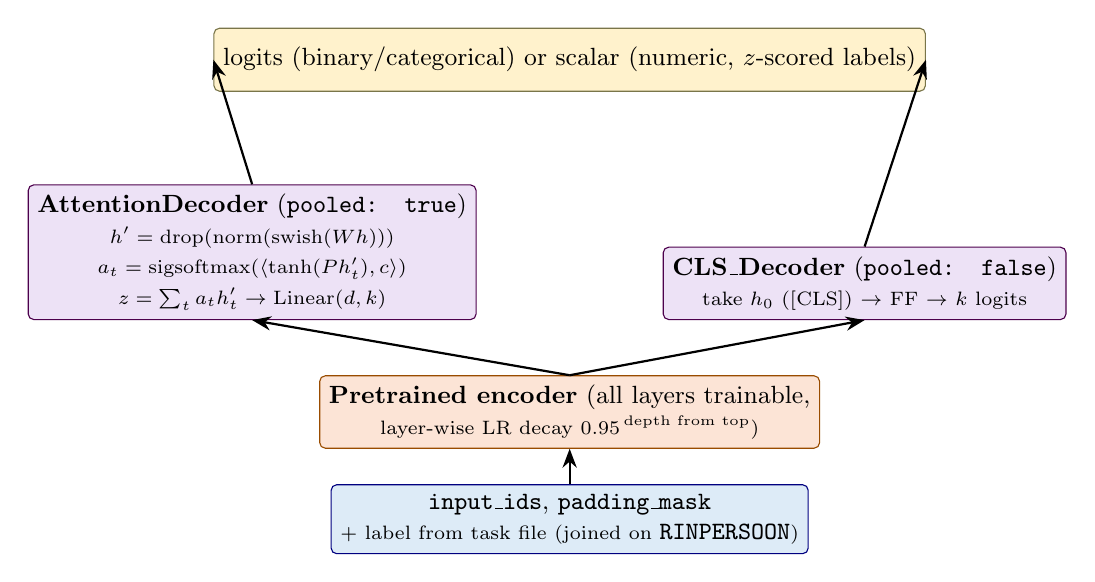
\begin{tikzpicture}[node distance=4.5mm and 10mm]
  \node[data] (in) {\code{input\_ids}, \code{padding\_mask}\\ \scriptsize + label from task file (joined on \code{RINPERSOON})};
  \node[model, above=of in, minimum width=56mm] (enc) {\textbf{Pretrained encoder} (all layers trainable,\\ \scriptsize layer-wise LR decay $0.95^{\,\text{depth from top}}$)};
  \node[head, above left=7mm and -20mm of enc] (attn) {\textbf{AttentionDecoder} (\code{pooled: true})\\
    \scriptsize $h'=\mathrm{drop}(\mathrm{norm}(\mathrm{swish}(Wh)))$\\
    \scriptsize $a_t = \mathrm{sigsoftmax}(\langle \tanh(P h'_t), c\rangle)$\\
    \scriptsize $z = \sum_t a_t h'_t \to \mathrm{Linear}(d,k)$};
  \node[head, above right=7mm and -20mm of enc] (cls) {\textbf{CLS\_Decoder} (\code{pooled: false})\\
    \scriptsize take $h_0$ ([CLS]) $\to$ FF $\to$ $k$ logits};
  \node[loss, above=36mm of enc, minimum width=50mm] (out) {logits (binary/categorical) or scalar (numeric, $z$-scored labels)};
  \draw[arr] (in) -- (enc);
  \draw[arr] (enc.north) -- (attn.south);
  \draw[arr] (enc.north) -- (cls.south);
  \draw[arr] (attn.north) -- (out.west);
  \draw[arr] (cls.north) -- (out.east);
\end{tikzpicture}
\caption{\code{TransformerFT}: pretrained encoder + lightweight task head. The
default head (\code{pooled: true}) is a learned attention pooling over all
token positions; the alternative uses the \code{[CLS]} vector only.}
\label{fig:ft}
\end{figure}

\subsection{Training recipe (per target column)}
\code{finetune\_runner.py} loops over the targets in the config and, for each:
\begin{enumerate}[nosep]
  \item Builds \code{FineTuneLazyDataset} train/val loaders (labels from
        \code{train\_path}/\code{val\_path}; optional
        \code{balance\_dataset} oversampling via \code{WeightedRandomSampler};
        optional Effective-Number weighting via the
        \code{class-balanced-loss} flag). Numeric targets
        are $z$-scored with train-set $\mu,\sigma$ (stored in hparams and
        inverted at evaluation).
  \item Optimizer: AdamW with \textbf{discriminative learning rates} ---
        embeddings get $lr \cdot 0.95^{n}$, encoder layer $i$ gets
        $lr \cdot 0.95^{\,n-i-1}$, the head gets $2\,lr$; OneCycle schedule;
        early stopping (patience 3) and checkpointing on \code{val\_auc\_epoch}
        (classification) or \code{val\_r2\_epoch} (numeric).
  \item \textbf{Binary threshold}: at each validation epoch end, probabilities
        are all-gathered across GPUs and the exact best-F1 threshold is found;
        after training, the threshold from the best checkpoint's validation
        pass is written \emph{into the checkpoint file} (\code{best\_thr}), so
        test-time predictions are consistent.
  \item In \code{test\_only} mode, the saved checkpoint is loaded and
        \code{trainer.predict} runs over the test HDF5 rows; predictions are
        all-gathered, metrics computed against the test label file, and
        (optionally) per-person prediction CSVs written. A ``safe dataset''
        wrapper replaces any out-of-vocabulary token id with PAD as a guard
        against vocab mismatches between checkpoint and data.
\end{enumerate}
Results go to the \emph{same} CSV schema as \file{train\_simple.py}
(Fig.~\ref{fig:pipeline}), which is what makes static vs.\ finetuned comparisons
one-liner joins.

% =====================================================================
\section{Static vs.\ Finetuned, Side by Side}
% =====================================================================

\begin{center}\small
\begin{tabular}{@{}p{3.4cm}p{5.4cm}p{5.4cm}@{}}
\toprule
 & \textbf{Static (2a $\to$ 3a)} & \textbf{Finetuned (2b)} \\
\midrule
Scripts & \file{infer\_embedding.py} $\to$ \file{train\_simple.py} & \file{finetune\_runner.py} \\
Encoder weights & frozen (inference only) & all trainable (layer-wise LR decay) \\
Person representation & one pooled vector (mean or attention-weighted), computed once & attention-pooled or [CLS], recomputed and adapted per task \\
Predictor & 2-layer MLP on the vector & head on top of full encoder \\
Cost per new task & minutes (embeddings are cached) & full GPU training run per target \\
Class imbalance & Effective-Number loss weights & oversampling and/or EN weights \\
Binary threshold & best-F1 sweep on val, stored in \code{best\_thr} & same mechanism, stored in Lightning ckpt \\
Output & shared results CSV (+ prob/label CSVs) & shared results CSV (+ prediction CSVs) \\
\bottomrule
\end{tabular}
\end{center}

\noindent Intuition for when each wins: the static route measures what the
pretrained representation \emph{already contains}; the finetuned route measures
what the architecture can \emph{extract when optimized for the task}. Running
both on the same targets (identical CSV schema) is exactly how the codebase is
set up to quantify that gap.

% =====================================================================
\section{File Map and Config Cheat-Sheet}
% =====================================================================

\subsection{Who does what}
\begin{center}\small
\begin{tabular}{@{}lp{9.2cm}@{}}
\toprule
\textbf{File (under \code{pop2vec/llm/src/})} & \textbf{Role} \\
\midrule
\code{new\_code/preprocess\_data.py}    & clean raw tables; percentile-bin numerics; cap categoricals \\
\code{new\_code/create\_life\_seq\_parquets.py} & assemble per-person event sequences \\
\code{new\_code/pipeline.py}            & vocab creation; tokenize; offline MLM masking; write HDF5 \\
\code{tasks/mlm.py}                     & \code{encode\_document}: prefix, truncation, 4-stream tensor, 80/10/10 masking, CLS permutation task \\
\code{new\_code/load\_data.py}          & datasets (\code{CustomLazyHDF5Dataset}, \code{FineTuneLazyDataset}); \code{collate\_autoreg} (AR shift + death truncation) \\
\code{new\_code/pretrain.py}            & Step 1 launcher (Lightning) \\
\code{transformer/models.py}            & \code{TransformerEncoder}: losses, metrics, optimizer for \code{mlm} / \code{ar\_lm} \\
\code{transformer/transformer.py}       & encoder stack; MLM/CLS heads; finetune forward variants \\
\code{transformer/transformer\_utils.py}& \code{EncoderLayer}, ReZero/ScaleNorm/Gate, FFN \\
\code{transformer/embeddings.py}        & token + Time2Vec(age, abspos) + segment embeddings \\
\code{transformer/attention.py}, \code{performer.py} & Performer FAVOR+ + local heads; approximate attention matrix; attention-weighted pooling \\
\code{new\_code/infer\_embedding.py}    & Step 2a: person embeddings $\to$ HDF5/parquet \\
\code{new\_code/train\_simple.py}       & Step 3a: MLP on frozen embeddings; results CSV \\
\code{new\_code/finetune\_runner.py}    & Step 2b driver: per-target training/testing, thresholds, CSV \\
\code{new\_code/finetune\_model.py}     & \code{TransformerFT}: encoder + head, layer-wise LR, metrics \\
\code{new\_code/generative\_infer*.py}  & (GPT extras) sampling continuations from \code{ar\_lm} models \\
\bottomrule
\end{tabular}
\end{center}

\subsection{Key config fields per step}
\begin{center}\small
\begin{tabular}{@{}lp{10.6cm}@{}}
\toprule
\textbf{Step} & \textbf{Required / notable keys} \\
\midrule
\file{pretrain.py} (hparams txt/yaml) &
\code{checkpoint\_dir}, \code{mlm\_path} (the HDF5), \code{vocab\_path},
\code{num\_val\_items}, \code{batch\_size}, \code{epochs};
\code{training\_task} (\code{mlm}$|$\code{ar\_lm}), \code{causal\_attn} (AR),
\code{resume\_from\_checkpoint}, \code{load\_model\_weights\_only} \\
\addlinespace[2pt]
\file{infer\_embedding.py} (JSON) &
\code{checkpoint\_path}, \code{tokenized\_path}, \code{emb\_write\_path};
\code{batch\_size}, \code{needed\_ids\_path}, \code{save\_token\_embs},
\code{use\_attention\_weighted\_emb} \\
\addlinespace[2pt]
\file{train\_simple.py} (JSON) &
\code{emb\_path}, \code{target\_column} = \{name: [type, $k$]\},
\code{task\_file}, \code{model\_name}, \code{result\_dir};
train mode: \code{train\_path}, \code{val\_path}, \code{model\_save\_dir};
test mode: \code{test\_only}, \code{test\_path}, \code{load\_model\_path};
optional \code{PARTNER\_KEY} (couple mode) \\
\addlinespace[2pt]
\file{finetune\_runner.py} (JSON) &
\code{sequence\_encoded} (HDF5), \code{task\_file}, \code{target\_column},
\code{result\_dir}; train: \code{train\_path}, \code{val\_path},
\code{model\_save\_dir}, \code{pretrained\_model\_path},
\code{pretrained\_model\_hparams}, \code{model\_name};
test: \code{test\_only}, \code{test\_path}, \code{load\_model\_path};
knobs: \code{pooled}, \code{balance\_dataset}, \code{class-balanced-loss},
\code{layer\_lr\_decay}, \code{devices}, \code{save\_predictions} \\
\bottomrule
\end{tabular}
\end{center}

% =====================================================================
\section{Frequently Confusing Points (Read This Twice)}
% =====================================================================
\begin{enumerate}[itemsep=2pt]
  \item \textbf{Masking is offline.} Unlike RoBERTa-style dynamic masking, the
    \code{[MASK]} pattern is fixed when \file{pipeline.py} writes the HDF5. The
    dataloader flag \code{mlm\_encoded} simply says ``this file contains the
    target columns'': it must be \code{True} for MLM pretraining and
    \code{False} for AR pretraining and for inference (which also flips on
    returning \code{sequence\_id}).
  \item \textbf{One encoder, two objectives.} \code{mlm} and \code{ar\_lm}
    share \code{Transformer} exactly; the differences live in the batch format
    (pre-masked vs.\ shifted), the head (gathered MLM decoder vs.\ full-sequence
    tied LM head), and \code{causal\_attn}. A checkpoint remembers its hparams,
    so \code{load\_from\_checkpoint} reconstructs the right variant
    automatically.
  \item \textbf{\code{input\_ids} is $(B,4,L)$, not $(B,L)$.} Row 0 = token ids,
    row 1 = abspos (days), row 2 = age, row 3 = segment. Everything downstream
    (\code{x[:,0]}, \code{x[:,1]}, \dots in \code{Transformer.forward}) depends
    on this order.
  \item \textbf{The val split is positional.} Validation = the \emph{first}
    \code{num\_val\_items} rows of the HDF5; randomness comes from the pipeline
    shuffling people at creation time. Keep \code{num\_val\_items} consistent
    between runs to compare losses.
  \item \textbf{Attention is approximate everywhere.} Full softmax attention is
    deliberately disabled; both training and the ``attention matrix'' used for
    attention-weighted embeddings are Performer approximations. The extracted
    importance scores come from the \emph{last} layer only.
  \item \textbf{Two different \code{train\_simple.py} exist} ---
    \code{new\_code/train\_simple.py} (documented here) and an earlier
    \code{evaluation/prediction\_settings/train\_simple.py} from which
    \code{finetune\_runner.py} imports \code{\_en\_weights}. They share the CSV
    schema and the MLP.
  \item \textbf{Binary decisions are threshold-tuned, not 0.5.} Both routes
    sweep validation probabilities for the F1-optimal threshold and persist it
    in the model file (\code{best\_thr}); test-time labels use that stored
    threshold.
  \item \textbf{Numeric targets are $z$-scored during finetuning.} Predictions
    are un-normalized with the stored $\mu,\sigma$ before computing MAE/$R^2$
    --- if you ever see wildly wrong scales, check that these made it into the
    checkpoint.
  \item \textbf{Death truncation only applies to AR.} MLM sequences keep
    everything within the time window; \code{collate\_autoreg} cuts at the first
    \code{[death]\_[death]} token because nothing after it should be generated.
\end{enumerate}

\vspace{4mm}
\noindent\emph{Reference: Savcisens et al., ``Using Sequences of Life-events to
Predict Human Lives'' (life2vec), arXiv:2306.03009. This codebase extends it
with the AR (GPT) objective, Performer attention with local heads,
attention-weighted static embeddings, and the dual static/finetuned evaluation
harness on Dutch registry data.}

\end{document}
